\chapter{Postup}
\label{5-postup}



\section{Postup 1 - pomocí nástrojů QGIS}

GTFS obsahuje povinný CSV soubor \textit{stops.txt}. Tento soubor obsahuje mimo
jiných polí také pole \textit{zone\_id}, který je při tvorbě tarifních pásem klíčový.
Verze GTFS Loaderu 1.0.0 soubor \textit{stops.txt} převádí do vektorové vrstvy
ve formě bodů. Z této bodové vrstvy byla vytvořena vektorová vrstva Voroného 
diagramů nástrojem \textit{Voroného polygony} v programu QGIS.
Vstupem do tohoto nástroje je vektorová vrstva stops a výstupem jsou právě Voroného polygony.

%toto možná dát do teoretické části
Voroného diagramy, někdy pod názvy jako Voroného teselace, Voroného dekompozice,
Thiessenovy polygony nebo Dirichletova teselace, podle definice představují
rozklad množiny bodů \textit{P} na \textit{n} uzavřených či 
otevřených oblastí \textit{V(p) = \{V(p\textsubscript{i}), V(p\textsubscript{2}), ...,
V(p\textsubscript{n})\}} takových, že každý bod
\textit{q} nálěžící množině \textit{V(p\textsubscript{i})} je blíže k bodu
\textit{p\textsubscript{i}} než k jakémukoliv
bodu \textit{p\textsubscript{j}} náležící množině\textit{P}. \cite{bayer}


\begin{figure}[H] \centering
    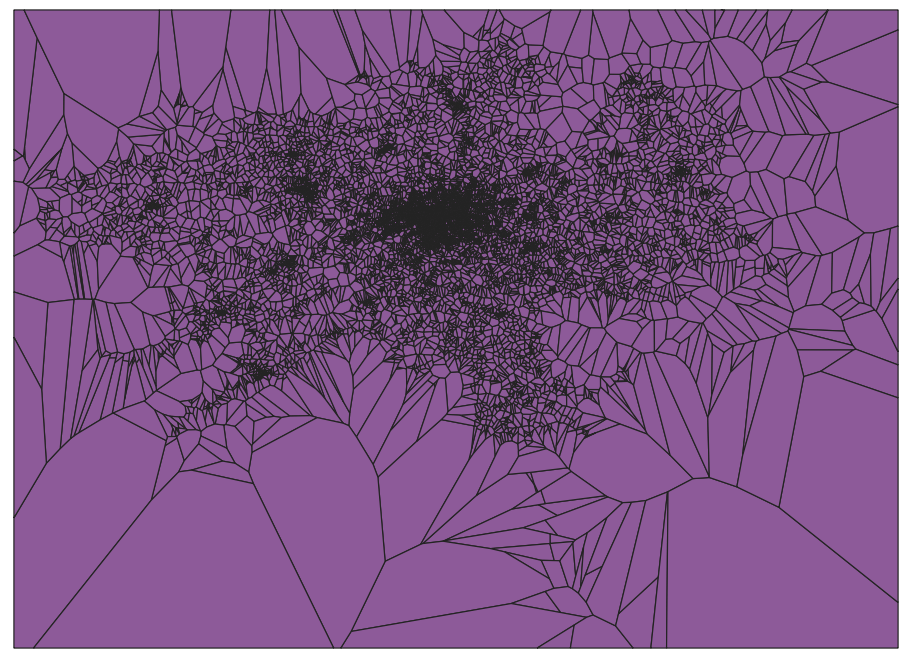
\includegraphics[width=400pt]{./pictures/voronoi.png}
    \caption[Voroného polygony]{Voroného polygony}
	\label{fig:voronoi}              
\end{figure}
%  
%  
% Poté přes nástroj Select by location vyberu ty polygony, které se prostorově protínají (Intersect) se zastávkami v požadovaném tarifním pásmu. Nástroj Select by location funguje na bázi prostorových dotazů. Jeho zdrojový kód je opět veřejně publikován na GitHubu. Vstupem do tohoto nástroje je vektorová vrstva stops a vektorová vrstva Voroného polygonů. Jako příklad zde budu uvádět tarifní pásmo 2. 
% Je důležité si uvědomit, že jsem vybral ty Voroného polygony, které protínají zastávky s tarifním pásmem 2. Poté totiž existují takové zastávky, které leží na hranicích tarifních pásem. Takové zastávky mají hodnotu pole zone_id například 1,2 nebo 2,3. Typ pole zone_id je proto String. 
% Vybrané Voroného polygony poté nástrojem Dissolve spojím do jednoho uceleného polygonu (viz obr. 7). Vstupem pro tento nástroj jsou vybrané Voroného polygony. Jeho zdrojový kód je opět veřejně publikován na GitHubu. 
% Ze spojených polygonů poté nástrojem Extract vertices vygeneruji vektorovou vrstvu bodů (viz obr. 8), které představují vrcholy spojených polygonů. Zdrojový kód je opět na GitHubu.
% 
% Obr. 8 Vrcholy spojených polygonů tarifního pásma 2
% Dále s SQL dotazy vyberu z původní vrstvy stops ty body, které mají hodnotu tarifního pásma 2, vytvořím novou vektorovou vrstvu a stejně tak pro body, které jsou na hranicích a mají hodnotu tarifního pásma 1,2 nebo 2,3. Tyto dvě vektorové funkce se spojí do jedné vrstvy spolu s vrstvou z Extract vertices (viz obr. 9). 
% 
% Obr. 9 Všechny body zahrnující se do tarifního pásma 2
% Z těchto spojených bodů již už vytvářím konkávní obálku. Na tu jsou v QGISu taktéž nástroje, buď Concave hull (alpha shapes) nebo Concave hull (k-nearest neighbor). Vyzkoušel jsem oba nástroje, ale výsledky se od sebe tolik nelišily. Concave hull (alpha shapes) vytváří pomocí Delaunay triangulací trojúhelníky mezi jednotlivými body. Poté se vyhledávají nejdelší hrany trojúhelníků, který se při tom násobí s konstantou alpha (threshold), která se volí v rozmezí 0-1, kde 1 je už konvexní obálka. Z hran trojúhelníků vzniknou polygony a nakonec se nástrojem Dissolve tyto polygony zcelí. Volí se i parametr, zda jsou či nejsou povoleny díry v polygonech, kde jsem já zaškrtnul, že nejsou povoleny. Podrobný postup lze vyčíst opět ze zdrojového kódu, který je opět na GitHubu. Concave hull (k-nearest neighbor) má mnohem komplexnější postup a je k naleznutí opět na GitHubu. Ve zkratce tam hlavně závisí na počtu sousedních bodů, které je třeba vzít v úvahu (nižší počet je konkávnější, vyšší počet je hladší).
% Dále jsem na výsledek konkávní obálky použil nástroj Simplify. Algoritmus poskytuje výběr metod zjednodušení, včetně vzdálenosti založené (algoritmus „Douglas-Peucker“), založené na ploše (algoritmus „Visvalingam“) a přichytávání geometrií k mřížce. Já jsem volil první metodu založenou na algoritmu „Douglas-Peucker“. Jako parametr se také volí Tolerance ve stupních, která je závislá na souřadnicovém systému a na velikosti vstupních dat. Zdrojový kód je k naleznutí opět na GitHubu.
% Výsledek není moc patrný, tak by mohlo stát za uvážení tento krok přeskakovat.
% Dalším nástrojem je Smooth. Tento nástroj používá algoritmus Chaikin, který vyhlazuje geometrie v liniové nebo polygonové vrstvě. Vytvoří novou vrstvu s vyhlazenými geometriemi obsahujícími vyšší počet vrcholů a rohů v geometriích. Na vstupu jsou parametry jako počet iterací, offset – zlomek linie k vytvoření nových vrcholů podél, volí se mezi 0 a 1 (například výchozí hodnota 0,25 vytvoří nové vrcholy 25% a 75% podél každého liniového segmentu geometrie pro každou iteraci, menší hodnoty mají za následek „těsnější“ vyhlazení) a poslední parametr maximální úhel v uzlu (0 - 180), pod kterým bude provedeno vyhlazení. Zdrojový kód je k naleznutí opět na GitHubu.
% 
% Obr. 12 Výsledek nástroje Smooth - 10 iterací, 0.25 offset, 180 max úhel v uzlu
% 
% Tento postup se provedl ve smyčce pro každé tarifní pásmo zvlášť. Tarifní pásma P, B a 0 byly brány jako jedno pásmo. Poté se provedl rozdíl vrstev nástrojem Difference, aby se vzájemně nepřekrývaly. Také se smazaly „ostrovní“ polygony menší než 50 km2, které byly oddělené od těch primárních výsledných polygonů. Nakonec se tyto vektorové vrstvy spojily do jedné vrstvy (viz obr. 13).
% Pokud to porovnáme s obr. 3, tak si můžeme všimnout, že výsledek sice tuto vektorovou vrstvu připomíná, ale rozhodně není ideální. Čím se to počítá dále od středu, tak se tvoří horší podoby těchto pásem. Navíc v postupu není zakomponováno „vyhýbání se“ zastavěných oblastí, což je podmínka od pracovníků z ROPIDu.
% Problém s hraničními zastávkami
% Největší problém však vidím s tzv. hraničními zastávkami neboli zastávkami, které leží na hranicích jednotlivých pásem a skrz tyto zastávky musí hranice procházet. Jak lze vidět na obr. 14, obr. 15, obr. 16 (pro každý obrázek nahoře – můj výsledek, dole – výsledek ROPIDu), tak můj postup tento problém vůbec neřeší, proto ho volím jako nevhodný pro výsledek mé diplomové práce. V postupu by se musel vyřešit již u konkávní obálky (v Concave hull (alpha shapes) u Delaunay triangulace), kde by se musel přetvořit její algoritmus o „povinné body“, přes které by to navíc konkávní obálku počítalo. Avšak nic takového mě zatím nenapadlo a nevím, jestli to je vůbec možné.  
% 
% 

